   \documentclass{report}
    \usepackage[letterpaper, portrait, margin=0.5in]{geometry}
    \usepackage[utf8]{inputenc}
    \usepackage{tikz}
    \usepackage{lipsum}
    \usepackage{mwe}
    \usetikzlibrary{graphs}
    \begin{document}
    \begin{figure}[htp]
    \centering
    \paragraph{\textsf{Rabin-Karp substring recurrance hashing}}
    \paragraph{ }
    \paragraph{ }
    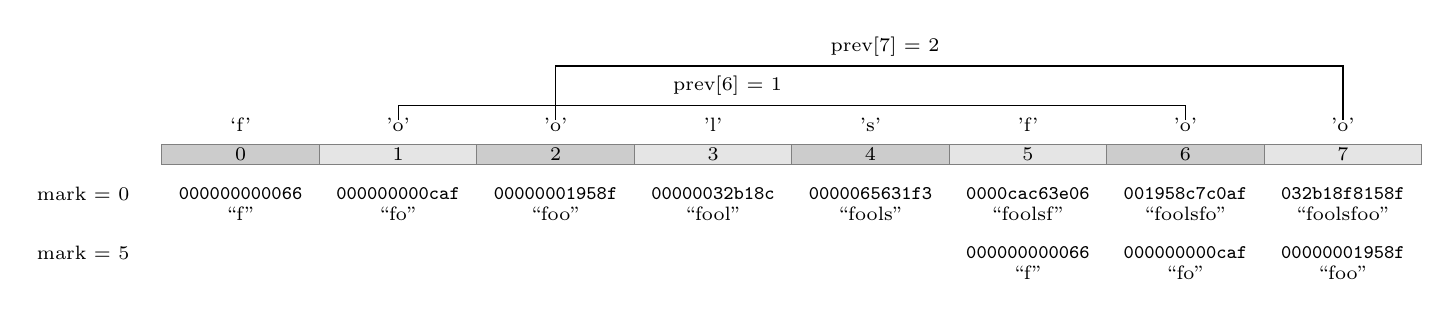
\begin{tikzpicture}[fill=blue!20,scale=0.250000]
    \begin{scope}[every node/.style={font=\scriptsize}]

\fill [black!20] (8,-1)    rectangle (0,-2);
\fill [black!10] (16,-1)   rectangle (8,-2);
\fill [black!20] (24,-1)   rectangle (16,-2);
\fill [black!10] (32,-1)   rectangle (24,-2);
\fill [black!20] (40,-1)   rectangle (32,-2);
\fill [black!10] (48,-1)   rectangle (40,-2);
\fill [black!20] (56,-1)   rectangle (48,-2);
\fill [black!10] (64,-1)   rectangle (56,-2);

\draw [black!50] (8,-1)    rectangle (0,-2);
\draw [black!50] (16,-1)   rectangle (8,-2);
\draw [black!50] (24,-1)   rectangle (16,-2);
\draw [black!50] (32,-1)   rectangle (24,-2);
\draw [black!50] (40,-1)   rectangle (32,-2);
\draw [black!50] (48,-1)   rectangle (40,-2);
\draw [black!50] (56,-1)   rectangle (48,-2);
\draw [black!50] (64,-1)   rectangle (56,-2);

\draw (60.0,0.25) -- (60.0,3.0) -- node[above left, pos=0.5]{prev[7] = 2} (20.0,3.0) -- (20.0,0.25);
\draw (52.0,0.25) -- (52.0,1.0) -- node[above left, pos=0.5]{prev[6] = 1} (12.0,1.0) -- (12.0,0.25);

\node (byte_0)     at ( 4.0 ,0.0) {`f'};
\node (byte_1)     at (12.0 ,0.0) {'o'};
\node (byte_2)     at (20.0 ,0.0) {'o'};
\node (byte_3)     at (28.0 ,0.0) {'l'};
\node (byte_4)     at (36.0 ,0.0) {'s'};
\node (byte_5)     at (44.0 ,0.0) {'f'};
\node (byte_6)     at (52.0 ,0.0) {'o'};
\node (byte_7)     at (60.0 ,0.0) {'o'};

\node (bit_63)    at ( 4.0  ,-1.5) {$0$};
\node (bit_63)    at (12.0  ,-1.5) {$1$};
\node (bit_63)    at (20.0  ,-1.5) {$2$};
\node (bit_63)    at (28.0  ,-1.5) {$3$};
\node (bit_63)    at (36.0  ,-1.5) {$4$};
\node (bit_63)    at (44.0  ,-1.5) {$5$};
\node (bit_63)    at (52.0  ,-1.5) {$6$};
\node (bit_63)    at (60.0  ,-1.5) {$7$};

\node (bit_63)    at (-4.0  ,-3.5) {mark = 0};
\node (bit_63)    at ( 4.0  ,-3.5) {\texttt{000000000066}};
\node (bit_63)    at (12.0  ,-3.5) {\texttt{000000000caf}};
\node (bit_63)    at (20.0  ,-3.5) {\texttt{00000001958f}};
\node (bit_63)    at (28.0  ,-3.5) {\texttt{00000032b18c}};
\node (bit_63)    at (36.0  ,-3.5) {\texttt{0000065631f3}};
\node (bit_63)    at (44.0  ,-3.5) {\texttt{0000cac63e06}};
\node (bit_63)    at (52.0  ,-3.5) {\texttt{001958c7c0af}};
\node (bit_63)    at (60.0  ,-3.5) {\texttt{032b18f8158f}};
\node (bit_63)    at ( 4.0  ,-4.5) {``f''};
\node (bit_63)    at (12.0  ,-4.5) {``fo''};
\node (bit_63)    at (20.0  ,-4.5) {``foo''};
\node (bit_63)    at (28.0  ,-4.5) {``fool''};
\node (bit_63)    at (36.0  ,-4.5) {``fools''};
\node (bit_63)    at (44.0  ,-4.5) {``foolsf''};
\node (bit_63)    at (52.0  ,-4.5) {``foolsfo''};
\node (bit_63)    at (60.0  ,-4.5) {``foolsfoo''};

\node (bit_63)    at (-4.0  ,-6.5) {mark = 5};
\node (bit_63)    at (44.0  ,-6.5) {\texttt{000000000066}};
\node (bit_63)    at (52.0  ,-6.5) {\texttt{000000000caf}};
\node (bit_63)    at (60.0  ,-6.5) {\texttt{00000001958f}};
\node (bit_63)    at (44.0  ,-7.5) {``f''};
\node (bit_63)    at (52.0  ,-7.5) {``fo''};
\node (bit_63)    at (60.0  ,-7.5) {``foo''};

    \end{scope}
    \end{tikzpicture}
    \end{figure}
    \end{document}
